
%(BEGIN_QUESTION)
% Copyright 2006, Tony R. Kuphaldt, released under the Creative Commons Attribution License (v 1.0)
% This means you may do almost anything with this work of mine, so long as you give me proper credit

Noen differansetrykktransmittere er utstyrt med \textit{femventilsmanifold}.  Disse ventilnettene muliggjør blokkering, utjevning og avlufting av transmitterens to trykkporter, med ventilene arrangert slik:

$$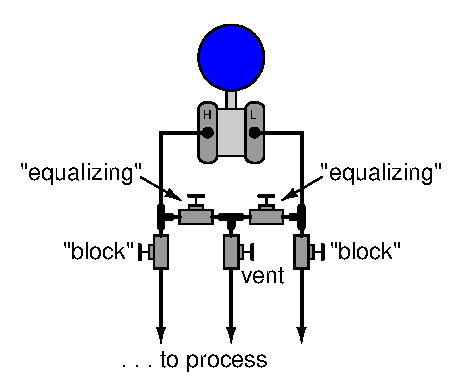
\includegraphics[width=15.5cm]{i00212x01.eps}$$

Vist med standard P\&ID-symboler ser transmitter/manifold-oppsettet slik ut:

$$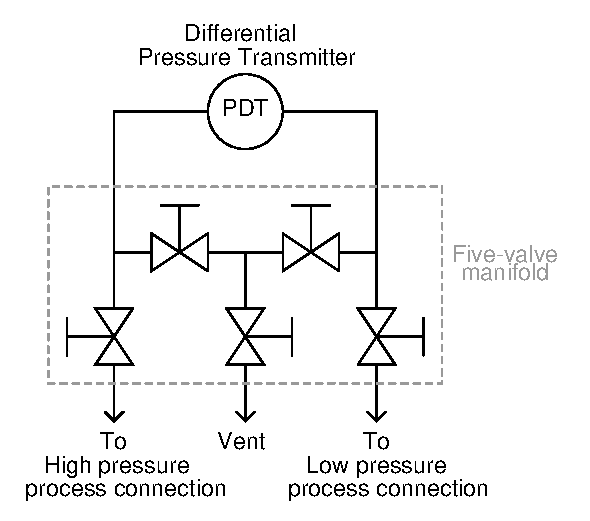
\includegraphics[width=15.5cm]{i00212x02.eps}$$

Identifiser normal ventilstatus (åpen/lukket) for femventilsmanifold.  Beskriv riktig ventilsekvens for å forberede transmitter for demontering.

\vskip 10pt

Hvorfor tror du vi bruker 5-ventilsmanifolder?  Hva kan gjøres med denne manifolden som ikke kan gjøres med en treventilsmanifold?

\underbar{file i00212}
%(END_QUESTION)





%(BEGIN_ANSWER)

Normal ventilstilling:

\begin{itemize}
\item{} Begge block-ventiler åpne.
\item{} Begge equalizing-ventiler lukket.
\item{} Vent-ventil lukket.
\end{itemize}

\vskip 10pt

Ta differansetrykktransmitter ut av drift:

\begin{itemize}
\item{} Lukk én block-ventil.
\item{} Åpne begge equalizing-ventiler (rekkefølgen mellom disse to er ikke kritisk).
\item{} Lukk den andre block-ventilen.
\item{} Åpne vent-ventilen.
\item{} Merk alle ventiler med informasjon om planlagt returtidspunkt.
\item{} Koble transmitteren fra manifolden.
\end{itemize}

\vskip 10pt

For å sette transmitteren tilbake i drift gjøres stegene i omvendt rekkefølge.

En fordel med 5-ventilsmanifold fremfor 3-ventilsmanifold er at ventlinjen kan føres til et fjernere og tryggere avluftingspunkt, nyttig for spesielt farlige prosessmedier.

Femventilsmanifold muliggjør også in-place kalibrering når én side av DP-transmitteren kan ventileres mot atmosfære.  Ved å koble kalibreringstrykk til ventlinjen kan trykket rutes til én side av transmitteren om gangen mens den andre siden er ventet.

%(END_ANSWER)





%(BEGIN_NOTES)


%INDEX% Safety, isolation valves: 5-valve equalizing manifold

%(END_NOTES)

